\documentclass{article}
% \usepackage{hyperref}

\usepackage{titlesec}
\usepackage{titling}
\usepackage{multicol}
% \usepackage{hyperref}
\usepackage[margin=0.2in]{geometry}

\usepackage{MnSymbol}
\usepackage{amsmath} 
\usepackage{graphicx} 
\usepackage{eso-pic}
\usepackage[hidelinks]{hyperref}

\hypersetup{
    colorlinks=true,
    linkcolor=blue,
    filecolor=magenta,      
    urlcolor=[rgb]{0,0,1},
    pdftitle={Kaustav-Resume},
    pdfpagemode=FullScreen,
    }


\usepackage{ifthen}
\newboolean{showProjectlinks}
\setboolean{showProjectlinks}{true}


\titleformat{\section}
{\large\uppercase}
{}
{0em}
{}[\titlerule]

\titleformat{\subsection}[runin]
{\bfseries}
{}
{1em}
{}[]

% \renewcommand{\maketitle}{
%     \begin{flushleft}        
%         {\huge\rmfamily
%         \theauthor}\newline
%         \vspace{0.1em}
%         \textit{teetangh@gmail.com -- github.com/teetangh}\newline
%         \textit{Contact No. -- +91-8800441954}\newline
%         \textit{Manipal Institute of Technology}\newline
%         \textit{B.Tech in \textbf{Computer Science \& Engineering}}
%         \textit{2018 - 2022}\newline
%         \textit{Minor in \textbf{Computational Intelligence}}\newline
%         \textit{CGPA: 8.51/10}\newline
%     \end{flushleft}
% }


\titlespacing*{\subsection}
{0em}
{0em}
{0em}


%%%%%%%%%%%%%%%%%%%%%%%%%%%%%%%%%%%%%%   DOCUMENT  %%%%%%%%%%%%%%%%%%%%%%%%%%%%%%%%%%%%%%%%%%%%%%%%%%%%%%%


\begin{document}
\thispagestyle{empty}  % for no page numbering

% \begin{multicols}{2}
%     \title{Resume}
%     \author{Kaustav Ghosh}
%     \maketitle
%     \begin{flushright}
%         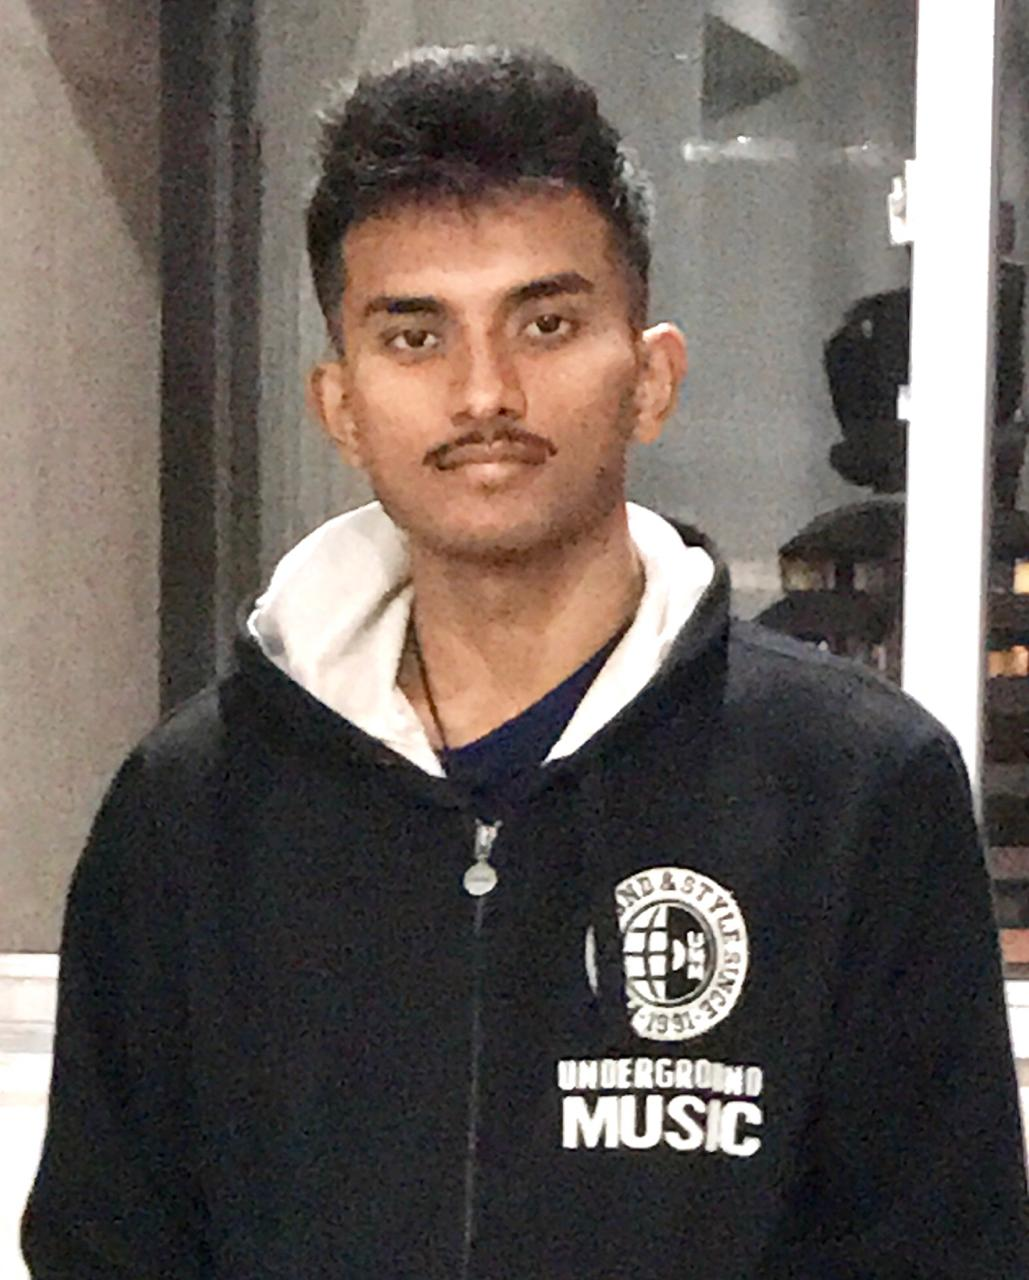
\includegraphics[height=3cm]{kaustav2.jpeg}
%     \end{flushright}
% \end{multicols}

\begin{center}
    \huge{Kaustav Ghosh}

    \normalsize{
        \textit{
            \href{https://www.github.com/teetangh}{GitHub} \(|\)
            \href{https://www.linkedin.com/in/kaustav-ghosh-1538651bb/}{LinkedIn} \(|\)
            teetangh@gmail.com \(|\)
            Gugraon,India \(|\)
            +91-8800441954
        }}
\end{center}

\section*{Education}
% \subsection*{
%     Manipal Institute of Technology
%     \begin{flushright}
%         \text{2018-2022}
%     \end{flushright}
%     }
% Left \hfill Center \hfill Right

\textbf{Manipal Institute of Technology} \hfill \textit{2018-2022}
\textmd{\newline \textit{BTech in Computer Science \& Engineering specializing in Computational Intelligence}} \hfill \textit{CGPA: 8.51/10}
\textmd{\newline \textit{Interests: Artificial Intelligence and Robotics}}
\ifthenelse{\boolean{showProjectlinks}}{\textbf{Lab Work:}
    \href{https://github.com/teetangh/Kaustav-CSE-LABS-and-Projects}{\text{[Repository]}}.
}{}



\section*{Work Experience}

\begin{itemize}
    \item{\textbf{\large{Samsung R\&D, Bangalore - Software Engineer Intern, IoT Products \& Analytics}}} \hfill \textit{Jun'21-Jul'21}
          \newline
          \textit{- Developed and implemented MQTT bridge functionality in Moquette, an open-source lightweight Java MQTT broker}
\end{itemize}


\begin{itemize}
    \item{\textbf{\large{Microsoft Student Partners-Machine Learning Intern}}} \hfill \textit{Apr'20-Jun'20}
          \newline
          \textit{-Guided a team of 10 individuals to collaborate and accomplish a Regression task of price prediction of used cars in a machine learning pipeline through Exploratory Data Analysis,Feature Engineering and Model Building.}
          \ifthenelse{\boolean{showProjectlinks}}{
              \textbf{Projects:}\href{https://nbviewer.jupyter.org/github/teetangh/Microsoft-Student-Partners-Machine-Learning-Internship/blob/main/MINOR\%20PROJECT/Microsoft_Minor_Project_v2.ipynb}{\text{[Minor]}}.
              \href{https://nbviewer.jupyter.org/github/Microsoft-ML-Internship-Team/Major-Project-Submissions/tree/master/KAUSTAV/}{\text{[Major]}}.
          }{}

\end{itemize}


% \begin{itemize}
%     \item{\textbf{\large{Qbotics Labs - ROS Engineer Intern}}}\hfill \textit{Jul'20-Aug'20}
%           \newline
%           \textit{- Constructed a Differential Drive with caster wheel from scratch using URDF \& XACRO files and mounted the same with laser scanner, IMU and Velodyne Puck VLP-16 Lidar and simulated the same in Gazebo and Webots}
%           \ifthenelse{\boolean{showProjectlinks}}{\textbf{Project:}
%               \href{https://github.com/teetangh/Qbotics-Labs-Internship-Differential-Drives}{\text{[Repository]}}.
%           }{}
% \end{itemize}


\begin{itemize}
    \item{\textbf{\large{TakenMind Technologies - Data Analytics Intern}}}\hfill \textit{May'20}
          \newline
          \textit{- Worked on analysing Industrial Data, predicting and presenting trends, using techniques such as Exploratory Data Analysis and Data visualisation using Matplotlib and Seaborn.Implemented several barplots, heatmaps, etc on several datasets.Implemented Machine Learning Algorithms (such as Random Forests).Obtained 87\% test accuracy.}
          \ifthenelse{\boolean{showProjectlinks}}{\textbf{Code:}
              \href{https://nbviewer.jupyter.org/github/Kaggle-Workspace/UN-SDG-Takenmind-Internship-IBM-Employee-Attrition/blob/main/Major\%20Assignment/Predicition.ipynb}{\text{[Notebook]}}.
          }{}

\end{itemize}


% \begin{itemize}
%     \item{\textbf{\large{Ineuron Deep Learning with Masters in Computer Vision and Natural Language Processing}}}
%           \newline
%           \textit{- Postponed due to Covid Situation }
% \end{itemize}


\section*{Research Work}
\begin{itemize}
    \item{\textbf{\large{Samsung PRISM - Intelligent Ranking for Dynamic Restoration in Next Generation Wireless Networks}}} \hfill \textit{Sep'20-Mar'21}
          \newline
          \textit{- Implemented Machine Learning algorithms and Feature Engineering techniques to predict KPI values for eNodeB-s and consequently a ranking system
              to orderly restore them during network failure.}
\end{itemize}

\section*{Projects}
\begin{itemize}
    \item{\textbf{\large{Compiler Frontend for subset of C-Language}}}
          % Don't know why indentation is not working
          \newline
          \textit{- Coded a \textbf{Lexical Analyser} that extracts tokens from a C source file and a \textbf{Symbol Table Generator} to store information of identifiers and functions and a \textbf{Recursive Decent Parser} that semantically parses the grammar for subset of C-Language by analysing the tokens generated by a Lexical Analyser}
          \ifthenelse{\boolean{showProjectlinks}}{\textbf{Code:}
              \href{https://github.com/teetangh/Kaustav-CSE-LABS-and-Projects/blob/main/Sem05-Compiler-Design-LAB/LAB\%2004/lab04_symbol_table_lexical_analyser_complete.c}{\text{[Lexical Analyser + Symbol Table]}}.
              \href{https://github.com/teetangh/Kaustav-CSE-LABS-and-Projects/blob/main/Sem05-Compiler-Design-LAB/LAB\%200789/lab09_RDP_main.c}{\text{[Recursive Decent Parser]}}.
          }{}
    \item{\textbf{\large{Mini Games based on Backtracking}}}
          \newline
          \textit{- Coded a \textbf{Crossword Solver} that takes a 10*10 grid and word list and outputs a grid with the words accurately filled}
          \newline
          \textit{- Coded a \textbf{Sudoku Solver} that takes a partially filled 9*9 Sudoku grid and outputs a solution so that every row, column and nine 3x3 sub-grids contains exactly 1 instance of the digits from 1 to 9.}
          \ifthenelse{\boolean{showProjectlinks}}{\textbf{Code:}
              \href{https://github.com/teetangh/competitive-programming/blob/main/CodeZen/03\%20Algorithms\%20and\%20Competitive\%20Programming/11\%20Backtracking/prog004crosswordSolver.cpp}{\text{[Crossword Solver]}}.
              \href{https://github.com/teetangh/competitive-programming/blob/main/CodeChef/Public/Code\%20Marathon/sudokuSolver.cpp}{\text{[Sudoku Solver]}}.
          }{}

    \item{\textbf{\large{Finland Labs \& IIT Roorkee - Time Series Forecasting, Data Analysis and Web Scraping}}}
          % Don't know why indentation is not working
          \newline
          \textit{- Prepared a complete Data Analysis report on the World-wide COVID-19 attack statistics and used the Facebook's fbprophet Time-series Forecasting library to speculate the number of active corona victim cases in the upcoming days.}\newline
          \textit{- Created neural networks from scratch which facilitated in implementing a machine learning model to recognize the function of an XOR gate without explicitly being programmed.}\newline
          \textit{- Trained a Deep Learning model with TF2 and Keras API for MNIST Handwritten digit Recognition}
          \ifthenelse{\boolean{showProjectlinks}}{\textbf{Code:}
              \href{https://nbviewer.jupyter.org/github/teetangh/FinlandLabs-IITR-COVID-19-Analysis/tree/main
              }{\text{[Project]}}.
          }{}
    \item{\textbf{\large{Machine Learning and Deep Learning Algorithms Implementations}}}
          \newline
          \textit{- Implemented basic machine learning algorithms such as Linear Regression, K-Nearest Neighbours, Logistic Regression,K-Means Clustering from scratch without existing machine learning libraries.Implemented few gradient descent algorthims
          }
          \newline
          \ifthenelse{\boolean{showProjectlinks}}{\textbf{Code:}
              \href{https://github.com/teetangh/Kaustav-AI-workspace/tree/main/ML}{\text{[AI-workspace]}}.
              \href{https://nbviewer.jupyter.org/github/Kaggle-Workspace/Gradient-Descent-Algorithms/blob/main/Gradient-Descent-Algorithms.ipynb}{\text{[Gradient-Descent-Algorithms]}}.
          }{}


    \item{\textbf{\large{Kaggle - Advanced House Price Prediction Regreesion Techniques}}}
          \newline
          \textit{-With 79 explanatory variables describing (almost) every aspect of residential homes in Ames, Iowa, this competition challenges, predicted the final price of each home.}
          \ifthenelse{\boolean{showProjectlinks}}{\textbf{Repository:}
              \href{https://nbviewer.jupyter.org/github/Kaggle-Workspace/House-Prices-Advanced-Regression-Techniques/blob/main/src/linear_reg_eda.ipynb}{\text{[Project]}}.
          }{}
          % \item{\textbf{\large{Food Labs Robotics Startup Competition}}}
          %       \newline
          %       \textit{- Designed, modelled, constructed and
          %           Assembled a plethora of sensors and Robots across multiple software platforms like
          %           freeCad,Blender,Gazebo and also fabricated a Defense Building from scratch using Gazebo World Editor}
          %       \ifthenelse{\boolean{showProjectlinks}}{\textbf{Repository:}
          %           \href{https://github.com/teetangh/FoodLabs-ROS-Startup-Competition}{\text{[Project]}}.
          %       }{}
          % \item{\textbf{\large{Analysis of Selective Compliance Assembly Robot Arm and Modelling of T3R Robot}}}
          %       \newline
          %       \textit{- Computed DH parameters for the SCARA robot and used it to compute the Forward and Inverse Kinematics of the robot arm and also its Lagrange Euler Dynamics}
          %       \ifthenelse{\boolean{showProjectlinks}}{\textbf{Repository:}
          %           \href{https://github.com/teetangh/robotics-modelling-workspace}{\text{[Project]}}.
          %       }{}
\end{itemize}

% \section*{Positions of Responsibility}
% \textmd{Local Committee Member of IOSD(International Organization of Software Developers)}

% \section{Courses Taken}
% % \subsection*{}
% \textbf{Coding Ninjas}- Completed C++ \& Data Structures.Currently doing Algorithms \& Competitive Programming Course.
% \newline
% \textbf{NPTEL}-Basic Electronics,Switching Circuits \& Logic Design,Computer Organization \& Architecture,OOP with Java

\section*{Technical Section}
\subsection*{Softwares Used:}
AutoCAD,Matlab,Keil,Altera MaxPlus 2,VirtualBox,Vm Ware,Oracle SQL,GNS 3 Network Simulator
\subsection*{Programming Languages:}
Fluent in C/C++ \& Python ,Familiar with Java ,Verilog,{\LaTeX},Linux Shell Scripting
% , fair acquaintance with ARM assembly programming\textit{(NXP LPC 1768)}
\subsection*{Libraries \& Frameworks:}
\textbf{C++}-STL
\textbf{Java}-JavaFX GUI
\textbf{Python}-Numpy, Pandas, Scikit-Learn, Keras, Tensorflow, PyTorch
% \subsection*{Robotics Libraries \& Frameworks:}
% ROS middleware, Gazebo, Ignition, MoveIt!, Point Cloud Library
%\subsection*{Web-Dev Languages,Libraries \& Frameworks:}
%Fair acquaintance with HTML, CSS, JavaScript \& with MERN %stack
\subsection*{Operating Systems:}
\textbf{Windows}-XP,Vista,7,10
\textbf{Linux}-Ubuntu 18.04



\end{document}